%\vnegs
\section{Introduction}
%\vnegxxs

%\FloatBarrier
  \begin{wrapfigure}{r}{0.45\textwidth}
    \centering
    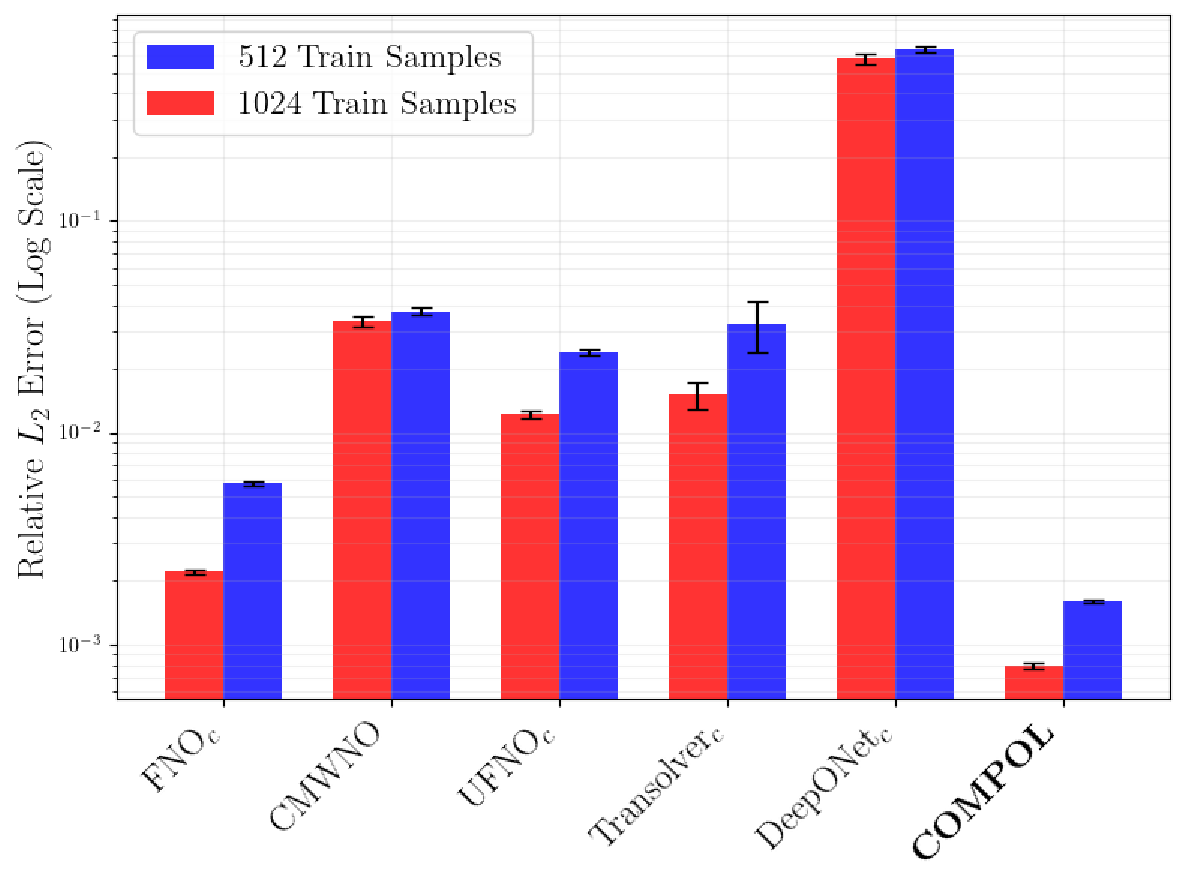
\includegraphics[width=0.45\textwidth]{figs/output.pdf}
    \caption{\footnotesize Predictive performance comparison of state-of-the-art neural operators vs. \ours on the 3-process Belousov–Zhabotinsky equations (512 and 1024 samples).}
  \end{wrapfigure}


Physical simulations governed by partial differential equations (PDEs) are fundamental tools across numerous scientific and engineering fields, including aerospace engineering, fluid mechanics, chemical processes, and environmental modeling~\citep{reed1980methods, arnol2013mathematical, evans2022partial,chorin1990mathematical, bergman2011fundamentals}. These simulations leverage core physical principles, such as conservation laws and symmetries, to accurately predict complex phenomena. Traditional numerical methods, like finite difference, finite element, and finite volume techniques, have been extensively used but face significant computational challenges when addressing high-dimensional or coupled multi-physics problems~\citep{quarteroni2010numerical, susanne1994mathematical,leveque2007finite, hughes2003finite}. Recent advances in machine learning have introduced neural operator methods ~\citep{kovachki2023neural, lu2021learning, li2020neural,li2020multipole}, notably the Fourier Neural Operator (FNO)~\citep{li2020fourier}, which directly approximate solution mappings between infinite-dimensional function spaces, significantly enhancing computational efficiency. Despite their promise, existing neural operator methods often inadequately capture the intricate correlations and dependencies present in coupled multi-physics systems.


Modeling multi-physics systems presents unique challenges due to the dynamic and complex interactions between multiple distinct physical processes, each governed by its own set of PDEs. These interactions often span multiple spatial and temporal scales, creating significant computational complexity and modeling difficulties~\citep{keyes2013multiphysics, quarteroni2009numerical}. Examples include fluid-structure interactions, chemical reaction-diffusion systems, and multiphase geological flows~\citep{bazilevs2013computational, bungartz2006fluid, weinan2003multiscale, cross2009pattern, holmes2012turbulence}, \etc Current neural operator frameworks typically treat these processes independently or apply overly simplistic coupling strategies, resulting in insufficient representation of inter-process dynamics. Consequently, capturing the nuanced interactions and accurately predicting system behaviors remains a critical and unresolved challenge in neural operator-based multi-physics modeling.

To address these challenges, we propose COMPOL, a novel coupled multi-physics operator learning framework explicitly designed to effectively represent complex interactions among multiple physical processes. COMPOL introduces sophisticated recurrent~\citep{cho2014learning} and attention~\citep{vaswani2017attention} mechanisms for latent feature aggregation, capturing detailed inter-process interactions within latent representation spaces. Notably, our proposed framework is architecture-agnostic, capable of integration with various neural operator frameworks that involve latent feature transformations. Our contributions are as follows:
\begin{itemize}
	\item  Proposing a versatile, architecture-agnostic operator learning framework tailored for coupled multi-physics systems, enhancing traditional operator layers with sophisticated feature aggregation methods.
	\item Introducing flexible latent aggregation techniques, including recurrent and attention mechanisms, to robustly capture dynamic inter-process dependencies.
	\item Demonstrating \ours's significant effectiveness and scalability across diverse multi-physics benchmarks, including predator-prey dynamics, chemical reactions, multiphase flows, and thermo-hydro-mechanical processes. Unlike previous methods restricted to coupling only two processes, COMPOL scales flexibly to an arbitrary number of interacting physical processes, consistently achieving substantial improvements in predictive accuracy compared to state-of-the-art approaches.
\end{itemize}
Collectively, \ours establishes a robust, flexible, and generalizable approach, significantly advancing the modeling capabilities of neural operators for complex multi-physics simulations.



 




%%experimental result

